% !TEX TS-program = pdflatex
% !TEX encoding = UTF-8 Unicode

\documentclass[11pt]{article} % use larger type; default would be 10pt

\usepackage[utf8]{inputenc} % set input encoding (not needed with XeLaTeX)

%%% PAGE DIMENSIONS
\usepackage[top=0.6in, left=0.8in, right=0.8in, bottom=0.7in]{geometry} % to change the page dimensions
\geometry{a4paper} % or letterpaper (US) or a5paper or....
% \geometry{margins=2in} % for example, change the margins to 2 inches all round
% \geometry{landscape} % set up the page for landscape

\usepackage{graphicx} % support the \includegraphics command and options

\usepackage[parfill]{parskip} % Activate to begin paragraphs with an empty line rather than an indent

%%% PACKAGES
\usepackage{booktabs} % for much better looking tables
\usepackage{array} % for better arrays (eg matrices) in maths
\usepackage{paralist} % very flexible & customisable lists (eg. enumerate/itemize, etc.)
\usepackage{verbatim} % adds environment for commenting out blocks of text & for better verbatim
\usepackage{subfig} % make it possible to include more than one captioned figure/table in a single float
\usepackage{mathtools} % for math environments like align
\usepackage{amssymb} % for symbols like \therefore
\usepackage{verbatim}
\usepackage{listings}
\usepackage{color}
\usepackage{overpic}

%%% OPTIONAL PACKAGES
%\usepackage{braket}

%%% HEADERS & FOOTERS
\usepackage{fancyhdr} % This should be set AFTER setting up the page geometry
\pagestyle{fancy} % options: empty , plain , fancy
\renewcommand{\headrulewidth}{0pt} % customise the layout...
\lhead{}\chead{}\rhead{}
\lfoot{}\cfoot{\thepage}\rfoot{}

%%% SECTION TITLE APPEARANCE
\usepackage{sectsty}
\allsectionsfont{\sffamily\mdseries\upshape} % (See the fntguide.pdf for font help)

\usepackage[svgnames]{xcolor}
\usepackage{tikz}
\usetikzlibrary{decorations.markings}
\usetikzlibrary{shapes.geometric}

\newif\iffinal % introduce a switch for draft vs. final document
\finaltrue % use this to compile the final document

\iffinal
  \newcommand{\inputTikZ}[1]{%
    \input{#1}%
  }
\else
  \newcommand{\inputTikZ}[1]{%
    \beginpgfgraphicnamed{#1-external}%
    \input{#1}%
    \endpgfgraphicnamed%
  }
\fi

%%% END Article customizations
\renewcommand{\d}{\,\mathrm{d}} % for integrals
\newcommand{\dx}[2]{\frac{\textrm{d} #1}{\textrm{d} #2}} % for derivatives
\newcommand{\dd}[2]{\frac{\textrm{d}^2 #1}{\textrm{d} #2^2}} % for double derivatives
\newcommand{\pd}[2]{\frac{\partial #1}{\partial #2}} % for partial derivatives
\newcommand{\pdd}[2]{\frac{\partial^2 #1}{\partial #2^2}} % for double partial derivatives
\newcommand{\e}[1]{\text{e}^{#1}} % for exponentials
\newcommand{\code}[1]{\texttt{#1}}
\newcommand{\inter}[1]{\shortintertext{#1}}

\begin{document}

  \begin{center}
    \vspace*{\fill}

    \centering
    
\includegraphics[scale=1.0]{Logo.pdf}
    \vfill

    \hrule
    {\LARGE\bf Year 3 C++ Project\\ E-Publication Document Creator \\[0.6cm]}
    \hrule 

    \vfill
    \large
    School of Physics and Astronomy\\
    University of Birmingham

    \vfill
    {\bf Josh Wainwright\\}
    UID:1079596
    \vfill

    \vfill
    Project Supervisor: Dr Steve Hillier\\
    Date: December 2012
    \vfill
    
    \vfill

  \end{center}

\newpage

\tableofcontents
\vspace{1cm}\hrule \vspace{1cm}
%\newpage
\section{Motivation}
This project is to build an application that aids in the creation of a simple ebook. Following the defined file structure, the user will have a number of options to customise the book, including title, author and date etc\., and choose the html files that make up the book and any images that are associated with it.

\section{Details}
The e-publication document format, or epub for short, is a free and open e-book standard created by the International Digital Publishing Forum (IDPF). It is designed to contain reflowable content which is content that can adapt its presentation depending on the device used to view it. This means that it is ideally suited for use by publishers on devices like e-book readers that have different sizes and means that some customisation by the user, like screen rotation and text size, is possible.

The epub document consists of the html, or similar, files that make up the text of the document and are referenced from a number of files required by the ebook-reader. These files are then wrapped in a ZIP archive along with the directory structure. The file structure is shown in figure \ref{fig:structure}.
\begin{figure}[ht]
  \centering
  \begin{tikzpicture}
    \node (0) at (0, 5) {e-Book};
    \node (1) at (2, 4.5) {mimetype};
    \node (3) at (2, 4) {META-INF};
    \node (6) at (2, 3) {OEPBS};
    \node (11) at (4, 3.5) {container.xml};
    \node (13) at (4, 0.5) {image files};
    \node (14) at (4, 1) {content html files};
    \node (15) at (4, 1.5) {title.html};
    \node (16) at (4, 2) {toc.ncx};
    \node (17) at (4, 2.5) {content.opf};
    \draw[dashed] (0) |- (1);
    \draw (0) |- (3);
    \draw (0) |- (6);
    \draw[dashed] (3) |- (11);
    \draw[dashed] (6) |- (13);
    \draw[dashed] (6) |- (14);
    \draw[dashed] (6) |- (15);
    \draw[dashed] (6) |- (16);
    \draw[dashed] (6) |- (17);
  \end{tikzpicture}
  \caption{\label{fig:structure}The required directory structure for an epub ebook. Files are shown with dotted lines.} 
\end{figure}


Each of the files included is required to exist by the reader, as long as that reader conforms to the standards of the format, but they contain information that will vary from book to book.

\section{Project}
\subsection{Graphical User Interface}
My implementation of an epub creator uses a single main window that is opened when the user starts the program, shown in figure \ref{fig:main}. From here the main details of the book can be entered.
% \begin{figure}[ht]
%   \centering
%   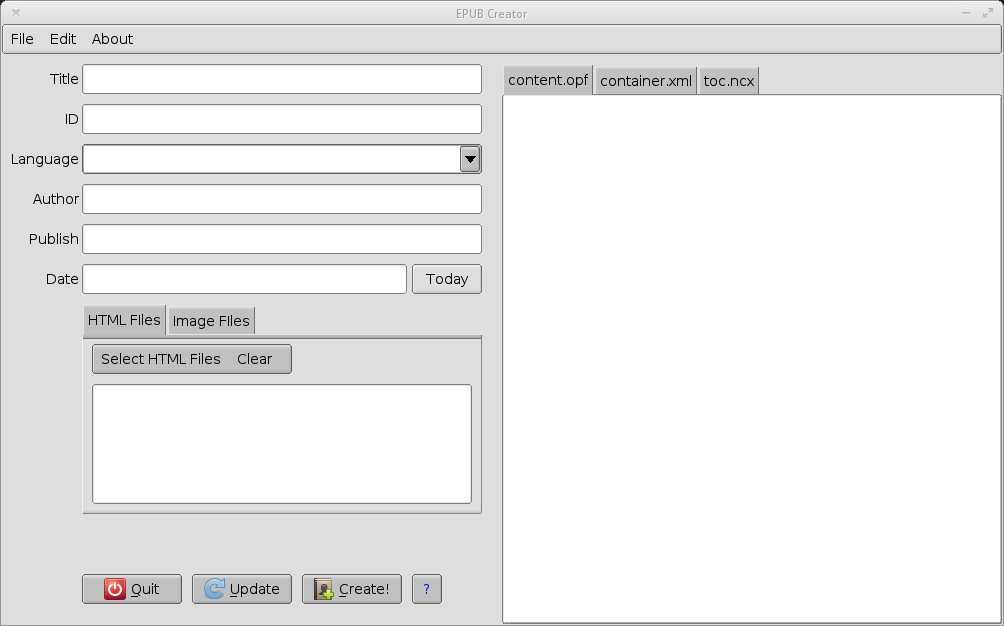
\includegraphics[width=0.9\columnwidth]{main.png}
%   \caption{\label{fig:main}The main window of the application that is shown when the program is started.} 
% \end{figure}

\begin{figure}[ht]
  \centering
  %\begin{overpic}[width=0.6\columnwidth,grid]{main.png}
  \begin{overpic}[width=0.6\columnwidth]{main.png}
    \put(-25,50){Input boxes}
    \put(-25,45){for book}
    \put(-25,40){details}
    \put(-5,45){\vector(3,4){7}}
    \put(-5,45){\vector(3,-4){7}}
    \put(-25,28){File selection}
    \put(-25,23){options}
    \put(-5,25){\vector(4,1){10}}
    \put(-25,7){Main control}
    \put(-25,2){buttons}
    \put(-5,4){\vector(1,0){10}}
    \put(105,30){Output windows}
  \end{overpic}
  \caption{\label{fig:main}The main window of the application that is shown when the program is started.}
\end{figure}

\begin{figure}[ht]
  \centering
  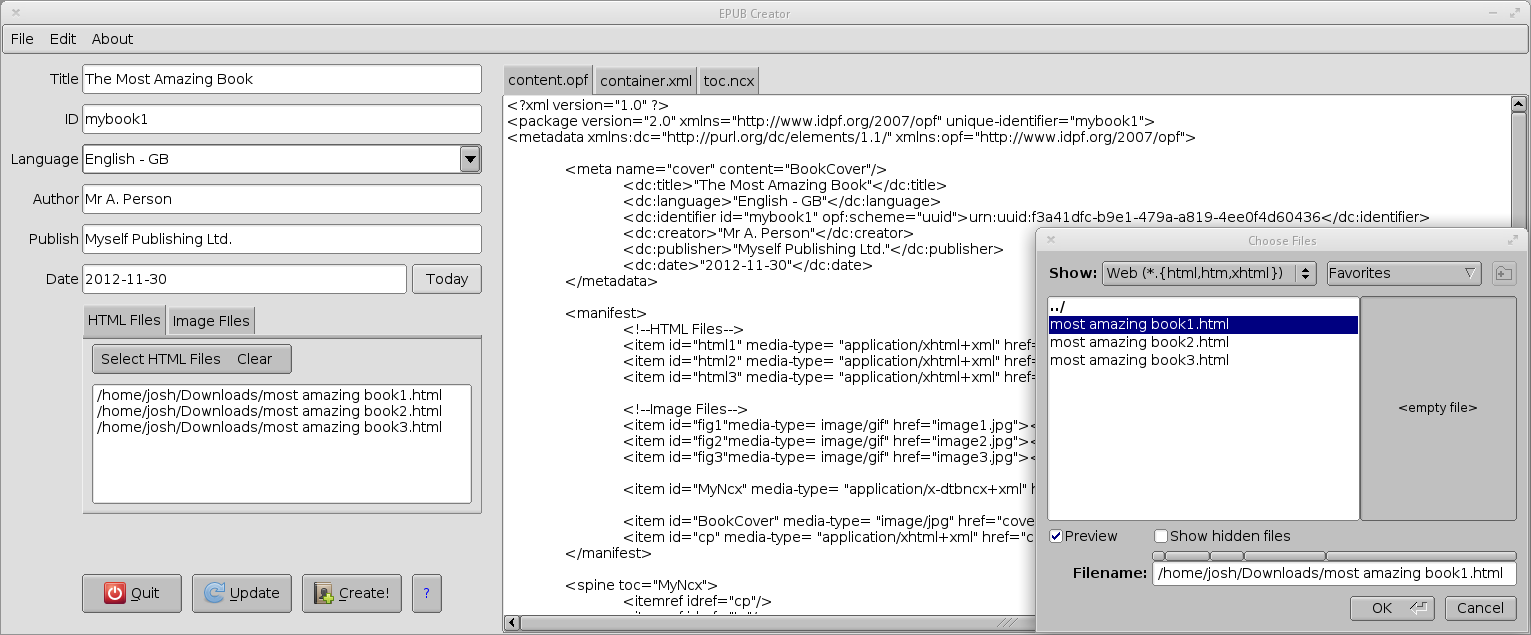
\includegraphics[width=0.9\columnwidth]{example.png}
  \caption{\label{fig:example}An example with the dialogue for choosing the html files to be included as well as an example of when data has been added to the relevant fields and the update button has been pressed to get a preview of the files.} 
\end{figure}

% \begin{figure}[ht]
%   \centering
%   % !TEX TS-program = pdflatex
% !TEX encoding = UTF-8 Unicode

\documentclass[11pt]{article}                                                   % use larger type; default would be 10pt
\usepackage[utf8]{inputenc}                                                     % set input encoding (not needed with XeLaTeX)

%%% PAGE DIMENSIONS ------------------------------------------------------------
\usepackage[top=0.8in, left=1in, right=1in, bottom=0.8in]{geometry}             % to change the page dimensions
\geometry{a4paper}                                                              % or letterpaper (US) or a5paper or....
\usepackage[parfill]{parskip}                                                   % Activate to begin paragraphs with an empty line rather than an indent

%%% HEADERS & FOOTERS ----------------------------------------------------------
\usepackage{fancyhdr}                                                           % This should be set AFTER setting up the page geometry
\pagestyle{fancy}                                                               % options: empty , plain , fancy
\renewcommand{\headrulewidth}{0pt}                                              % customise the layout...
\lhead{}\chead{}\rhead{}
\lfoot{}\cfoot{page \thepage}\rfoot{}

%%% SECTION TITLE APPEARANCE ---------------------------------------------------
\usepackage{sectsty}
\allsectionsfont{\sffamily\mdseries\upshape}                                    % (See the fntguide.pdf for font help)

%%% PACKAGES -------------------------------------------------------------------
\usepackage[font=small,labelfont=bf,textfont=it]{caption}                       % stylize captions
\usepackage{graphicx}                                                           % support the \includegraphics command and options
\usepackage{booktabs}                                                           % for much better looking tables
\usepackage{array}                                                              % for better arrays (eg matrices) in maths
\usepackage{paralist}                                                           % very flexible & customisable lists (eg. enumerate/itemize, etc.)
\usepackage{verbatim}                                                           % adds environment for commenting out blocks of text & for better verbatim
% \usepackage{subfig}                                                             % make it possible to include more than one captioned figure/table in a single float
\usepackage{mathtools}                                                          % for math environments like align
\usepackage{amssymb}                                                            % for symbols like \therefore
\usepackage{verbatim}                                                           % for including text as appears, verbatim
\usepackage{listings}                                                           % for including external files as text, eg code
\usepackage{color}                                                              % for coloring of files and images
\usepackage{overpic}                                                            % for adding annotations to pictures
\usepackage[version=3]{mhchem}
\usepackage{textcomp}
\usepackage{graphicx}
\usepackage{caption}
\usepackage{subcaption}

%%% EQUATIONS ------------------------------------------------------------------
\numberwithin{equation}{section}                                                % Number equations by section (change for different levels)

%% BIBIOGRAPHY ------------------------------------------------------------------
\usepackage{cite}
\bibliographystyle{unsrt}

%%% ToC (table of contents) APPEARANCE -----------------------------------------
%\usepackage[nottoc,notlof,notlot]{tocbibind}                                   % Put the bibliography in the ToC
%\usepackage[titles,subfigure]{tocloft}                                         % Alter the style of the Table of Contents
%\renewcommand{\cftsecfont}{\rmfamily\mdseries\upshape}
%\renewcommand{\cftsecpagefont}{\rmfamily\mdseries\upshape}                     % No bold!

%%% PDF LINKS AND STYLE --------------------------------------------------------
\usepackage[unicode=true,
    bookmarks=true,bookmarksnumbered=true,bookmarksopen=true,
    bookmarksopenlevel=2, breaklinks=false,pdfborder={0 0 0},backref=false,
    colorlinks=false] {hyperref}                                                % for links in pdf file, no colors
\hypersetup{pdftitle={DOCUMENT NAME},
    pdfauthor={Josh Wainwright}}                                                % set name of document and author here

%%% END Article customizations

\newcolumntype{L}{>{\centering\arraybackslash}m{3em}}
\newcolumntype{M}{>{\centering\arraybackslash}m{2em}}
\newcolumntype{N}{>{\centering\arraybackslash}m{5em}}
\newcolumntype{O}{>{\centering\arraybackslash}m{4em}}

%%% Include TIKZ images directly into document ---------------------------------
\usepackage[svgnames]{xcolor}
\usepackage{tikz}
\usetikzlibrary{decorations.markings}
\usetikzlibrary{shapes.geometric}

\newif\iffinal                                                                  % introduce a switch for draft vs. final document
\finaltrue                                                                      % use this to compile the final document
\usepackage{tikz}

\iffinal
    \newcommand{\inputTikZ}[1]{%
        \input{#1}%
    }
\else
    \newcommand{\inputTikZ}[1]{%
        \beginpgfgraphicnamed{#1-external}%
        \input{#1}%
        \endpgfgraphicnamed%
    }
\fi

%%% Include svg images directly in document (requires Inkscape) ----------------
\newcommand{\executeiffilenewer}[3]{%
    \ifnum\pdfstrcmp{\pdffilemoddate{#1}}%
        {\pdffilemoddate{#2}}>0%
        {\immediate\write18{#3}}
    \fi
}
\newcommand{\includesvg}[1]{%
    \executeiffilenewer{#1.svg}{#1.pdf}%
    {inkscape -z -D --file=#1.svg --export-pdf=#1.pdf --export-latex}%
    \input{#1.pdf_tex}%
}

%%% NEW COMMANDS ---------------------------------------------------------------
\renewcommand{\d}{\,\mathrm{d}}                                                 % for integrals
\newcommand{\dx}[2]{\frac{\textrm{d} #1}{\textrm{d} #2}}                        % for derivatives
\newcommand{\dd}[2]{\frac{\textrm{d}^2 #1}{\textrm{d} #2^2}}                    % for double derivatives
\newcommand{\pd}[2]{\frac{\partial #1}{\partial #2}}                            % for partial derivatives
\newcommand{\pdd}[2]{\frac{\partial^2 #1}{\partial #2^2}}                       % for double partial derivatives
\newcommand{\e}[1]{\text{e}^{#1}}                                               % for exponentials
\newcommand{\code}[1]{\texttt{#1}}                                              % for verbatim code view
\newcommand{\inter}[1]{\shortintertext{#1}}                                     % shorter version of intertext
\newcommand{\under}[1]{\underline{#1}}                                          % for vectors etc.

\let\vaccent=\v                                                                 % rename builtin command \v{} to \vaccent{}
\newcommand{\uv}[1]{\ensuremath{\hat{#1}}}                                      % for unit vector
\newcommand{\abs}[1]{\left| #1 \right|}                                         % for absolute value
\newcommand{\avg}[1]{\left< #1 \right>}                                         % for average
\let\underdot=\d                                                                % rename builtin command \d{} to \underdot{}
\newcommand{\ket}[1]{\left| #1 \right>}                                         % for Dirac bras
\newcommand{\bra}[1]{\left< #1 \right|}                                         % for Dirac kets
\newcommand{\braket}[2]{\left< #1 \vphantom{#2} \right|
    \left. #2 \vphantom{#1} \right>}                                            % for Dirac brackets
\newcommand{\matrixel}[3]{\left< #1 \vphantom{#2#3} \right|
    #2 \left| #3 \vphantom{#1#2} \right>}                                       % for Dirac matrix elements
\newcommand{\grad}[1]{\nabla #1}                                                % for gradient
\let\divsymb=\div                                                               % rename builtin command \div to \divsymb
\newcommand{\laplacian}[0]{\nabla^2}
\renewcommand{\div}[1]{\nabla \cdot \textbf{#1}}                                % for divergence
\newcommand{\curl}[1]{\nabla \times \textbf{#1}}                                % for curl
\let\baraccent=\=                                                               % rename builtin command \= to \baraccent
\renewcommand{\=}[1]{\stackrel{#1}{=}}                                          % for putting numbers above =


%*******************************************************************************
%******************************** END HEADER ***********************************
%*******************************************************************************

\begin{document}
%!TEX root = mainfile.tex
\begin{titlepage}
  \begin{center}
    \vspace*{\fill}

    \centering
    
\includegraphics[scale=1.0]{Logo.pdf}
    \vfill

    \hrule
    {\LARGE\bf Extragalactic Astrophysics and Cosmology\\Cosmic Reionization \\[0.4cm]}
    \hrule

    \vfill
    \large
    School of Physics and Astronomy\\
    University of Birmingham

    \vfill
    { Joe Baumber,
    	James Bryant,
    	Lewis Clegg,
    	Bethany Johnson,
    	Andrew King,
    	Owen McConnell,
    	Catherine McDonald,
    	Michael O'Neill,
    	Jonathan Shepley,
    	Dorothy Stonell,
    	Rahim Topadar,
    	Josh Wainwright\\}
    \vfill

    \vfill
    \textit{Supervisors:} Graham Smith, Alistair Sanderson, Melissa Gillone \\
    		\vfill
    \textit{Date:} March 2013
    \vfill
    \vfill

    \begin{abstract}
        This study deduces that reionization began at a redshift of $z=17.82$ and ended at a redshift of $z=7\pm 1.8$. This is calculated by directly applying the dynamics of star formation and the ionization rate of neutral hydrogen in the Intergalactic Medium. A photometry strategy consisting of 3 multi-band surveys is proposed in order to observe Lyman Break Galaxies across redshifts 6--17. The surveys will locate $100.5\pm37.0$, $138.7\pm 100.6$, $358.1\pm 158.6$ galaxies in redshift ranges 6--8.5, 8.5--10 and 10--17 respectively. These surveys will be completed by the James Webb Space Telescope and Euclid which are planned for launch in the coming decade. A follow up spectroscopy survey will be used to confirm the redshift and properties of 24, 4 and 48 galaxies in these 3 surveys respectively. The spectroscopy will be carried out using James Webb Space Telescope and a combination of single and multi-slit spectroscopy. It is shown that the use of known gravitational lenses, located between redshift 0.5--0.7, is very beneficial for discovering high redshift candidates as it can increase the depth of surveys by up to 3 magnitudes.
    \end{abstract}


  \end{center}
\end{titlepage}

%\thispagestyle{empty}
%\vspace*{\fill}
%\noindent
%\begin{tabular}{ll}
%\end{tabular}

%\cleardoublepage
%\cleardoublepage

\newpage
\tableofcontents
\newpage
%!TEX root = main.tex

\section{Introduction} % (fold)
\label{sec:introduction}
This experiment involves examining the interactions of neutrons with matter through two experiments using two different detectors. The first detector, a sodium iodide scintillation detector will be used to measure the binding energy of the neutron, and secondly, using a boron-trifluoride counter, measure the moderating properties of water on fast neutrons as a function of radius from a central source.
% section introduction (end)

%!TEX root = main.tex

\section{Neutron Binding Energy} % (fold)
\label{sec:neutron_binding_energy}

\subsection{Sodium Iodide Detector} % (fold)
\label{ssub:sodium_iodide_detector}
The first experiment that was performed involved using an NaI(Tl) detector. The sodium iodide detector is a scintillation detector that uses a NaI crystal doped with thallium to create scintillation photons when a gamma ray photon hits the crystal. The thallium is added as an activator to provide extra available energy levels that can be occupied by the photons in the crystal. In the pure state, the NaI has a large forbidden band gap between the conduction and valence bands, shown in figure~\ref{fig:thaliumactivator}. The activator reduces this gap so that an emitted photon is in the range that the photomultiplier tube is sensitive to, typically visible.
\begin{figure}[ht]
	\centering
	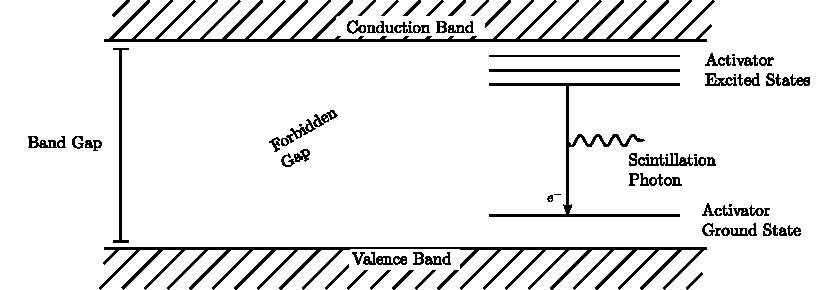
\includegraphics[width=0.9\textwidth]{NaIbands.pdf}
	\caption{The element thallium is added to the pure crystal of sodium iodide to provide extra energy levels for the electrons, which sit inside the forbidden gap of the crystal latice structure. These allow a photon of a useful wavelength to be emitted when electron decays to a lower energy.\label{fig:thaliumactivator}}
\end{figure}

When a gamma photon enters the detector it ionises a molecule of NaI creating excited states in the crystal that then decay via visible photons. The number of photons that are produced is proportional to the energy of the incident photon; as the energy of the gamma ray increases, more scintillation photons are produced. Thus, the energy of the original can be found be counting the number of photons produced. 

These scintillation photons are used to create electrons which are more easily counted. At the photo-cathode, the photons release electrons via the photoelectric effect. The electrons are then passed through the photomultiplier tube which increases the number of photons exponentially by accelerating them through a high potential difference so they can knock more electrons out from the dynodes (see figure~\ref{fig:naidetctor})\cite{krane}. This results in a stream of electrons that can be measured, and which is proportional to the original energy of the photon via the number of scintillation photons, the number of electrons and the multiplication factor of the increase of electrons from the PM tube. Since each of these steps is a simple relationship, a calibration setting can be taken using known results, and a simple equation relating the reading from the detector to the energy of the photon found.
\begin{figure}[ht]
	\centering
	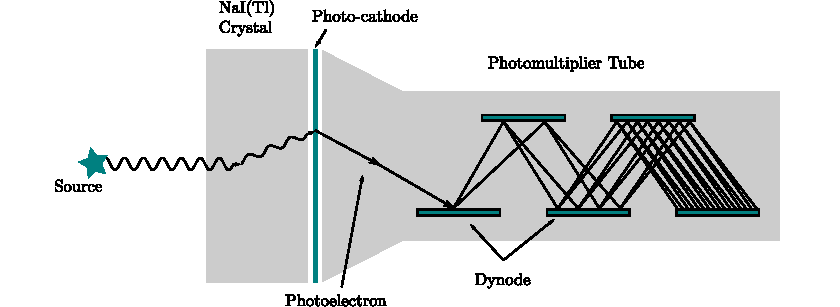
\includegraphics[width=0.9\textwidth]{NaIdetector.pdf}
	\caption{The sodium iodide detector is a commonly used gamma ray detector that uses the relationship between the energy of a photon and the ionisation power that it has to measure its energy via a calibration equation.\label{fig:naidetctor}}
\end{figure}

The detector requires a high voltage which is placed across the dynodes and the anode to accelerate the electrons once they have entered the PM tube. Using this method of acceleration and re-acceleration, the photomultiplier tube is able to increase the number of electrons by a factor of roughly $10^5$ depending on the voltage bias\cite{baratta}. For our experiment, a potential difference of 800 Volts was used. A schematic view of the experimental set-up is shown in figure~\ref{fig:experimentalsetp}.
\begin{figure}[ht]
	\centering
	\begin{tikzpicture}
    \node[rectangle, draw, text centered, text width=5em] (1) at (2,0) {NaI Scintillator};
	\node[rectangle, draw, text centered, text width=7em] (2) at (5,0) {Photomultiplier Tube};
	\node[rectangle, draw, text centered, text width=5em] (3) at (5,-2) {High Voltage};
	\node (4) at (7.81,0) {Pre-Amp};
	\node (tri1) at (6.9,1) {	};
	\node (tri2) at (9,0) {	};
	\node (tri3) at (6.9,-1) {};
	\draw (tri1.center) -- (tri2.center) -- (tri3.center) -- cycle;  
	\node[rectangle, draw] (5) at (11,0) {Oscilliscope};
	\node[rectangle, draw] (6) at (10,-2) {Amplifier};
	\node[rectangle, draw, text centered, text width=7em] (7) at (13,-2) {Multi Channel Analyser};
	\draw (1) -- (2);
	\draw[<-] (2) -- (3);
	\draw (2) -- (4);
	\draw[->] (tri2.center) -- (5);
	\draw (6) -| (tri2.center);
	\draw (6) -- (7);
	\draw[->] (7) |- (5);
\end{tikzpicture}
\caption{This diagram shows a schematic view of the set-up used with the sodium iodide detector. The amplifier is used on the side where the detector is connected to the computer simply to increase the level of the signal input to the computer so that it is at a readable level.\label{fig:experimentalsetp}}
\end{figure}

% subsubsection sodium_iodide_detector (end)

\subsection{Calibration} % (fold)
\label{sub:calibration}
Before any data can be read from the spectra taken from the detector, the data has to be calibrated. To do this, a set of known samples with well defined peaks is used to get a relation between the channel number of an observed peak and its energy. Once this is done, a relation can be found that relates the channel number to energy for use on later measurements.

The elements that were used included cobalt, barium, caesium, europium and americium. Each of these elements were available to measure, and each has recorded and accepted peaks that are at well defined positions. The data was taken from the National Nuclear Data Centre (NNDC)\cite{nndc}. The table below, table~\ref{tab:calibdata}, shows the data that we collected from these sources. The channel number refers to the position in the spectrum that the peak was observed and the expected peak is the energy of the peak that the respective peak is estimated to correspond to.

\begin{table}[ht]
	\centering
	\begin{tabular}{r c|c|c}
		\multicolumn{2}{c|}{Element} & Channel Number & Expected Peak Energy (keV) \\
		\hline\hline
		Cobolt 		& $\ce{^{60}Co}$  & 369.4	& 1332.0 \\
					&				  & 324.9	& 1173.0	\\
		\hline
		Barium		& $\ce{^{133}Ba}$ & 102.9	& 356.0	\\
					&				  & 86.08	& 302.9		\\
		\hline
		Caesium		& $\ce{^{137}Cs}$ & 188.4	& 661.7 \\
		\hline
		Europium	& $\ce{^{152}Eu}$ & 99.84	& 344.3 \\
					&				  & 222.0	& 778.9		\\
					&				  & 274.9	& 964.1		\\
					&				  & 311.0	& 1121/1086	\\
					&				  & 394.1	& 1408.0	
	\end{tabular}
	\caption{Several elements were used to measure a calibration relation that links the observed channel number to the energy.\label{tab:calibdata}}
\end{table}
From these, the graph in figure~\ref{fig:naicalib} can be drawn which shows the relation that can be used as a calibration between energy and channel number. The exact value of this relation, intercept and gradient, are subject to change since the calibration is retaken at the start of each session to account for changes in the experimental set-up and the radioactivity of the source which will decrease with time.

\begin{figure}[ht]
	\centering
	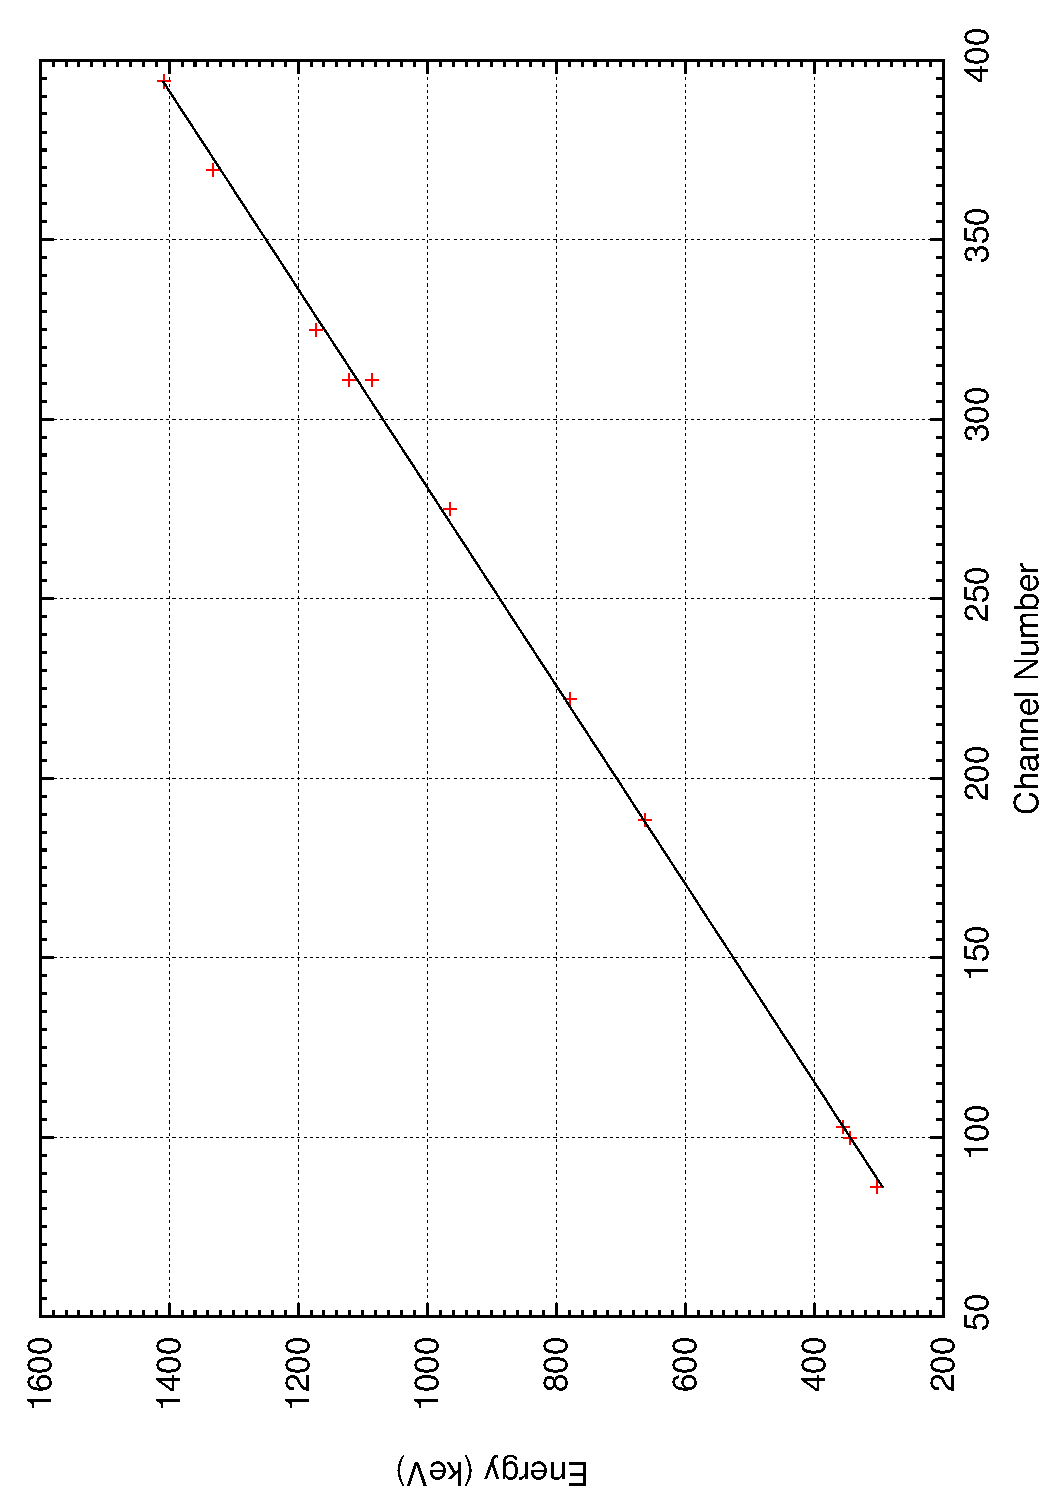
\includegraphics[angle=270,width=0.6\textwidth]{calibration1NaI.pdf}
	\caption{The sodium iodide detector provides a channel number readout that is directly proportional to the energy of the corresponding reaction event. Thus, using known data points, a relation between channel number and energy can be found.\label{fig:naicalib}}
\end{figure}
An example of the spectra from the sources is shown in figure~\ref{fig:cobaltcalib}. This shows the spectrum of $\ce{^{60}Co}$ which has been fitted with the Gaussian peaks to find the position and FWHM using the ``root'' package\cite{root}.

\begin{figure}[ht]
	\centering
	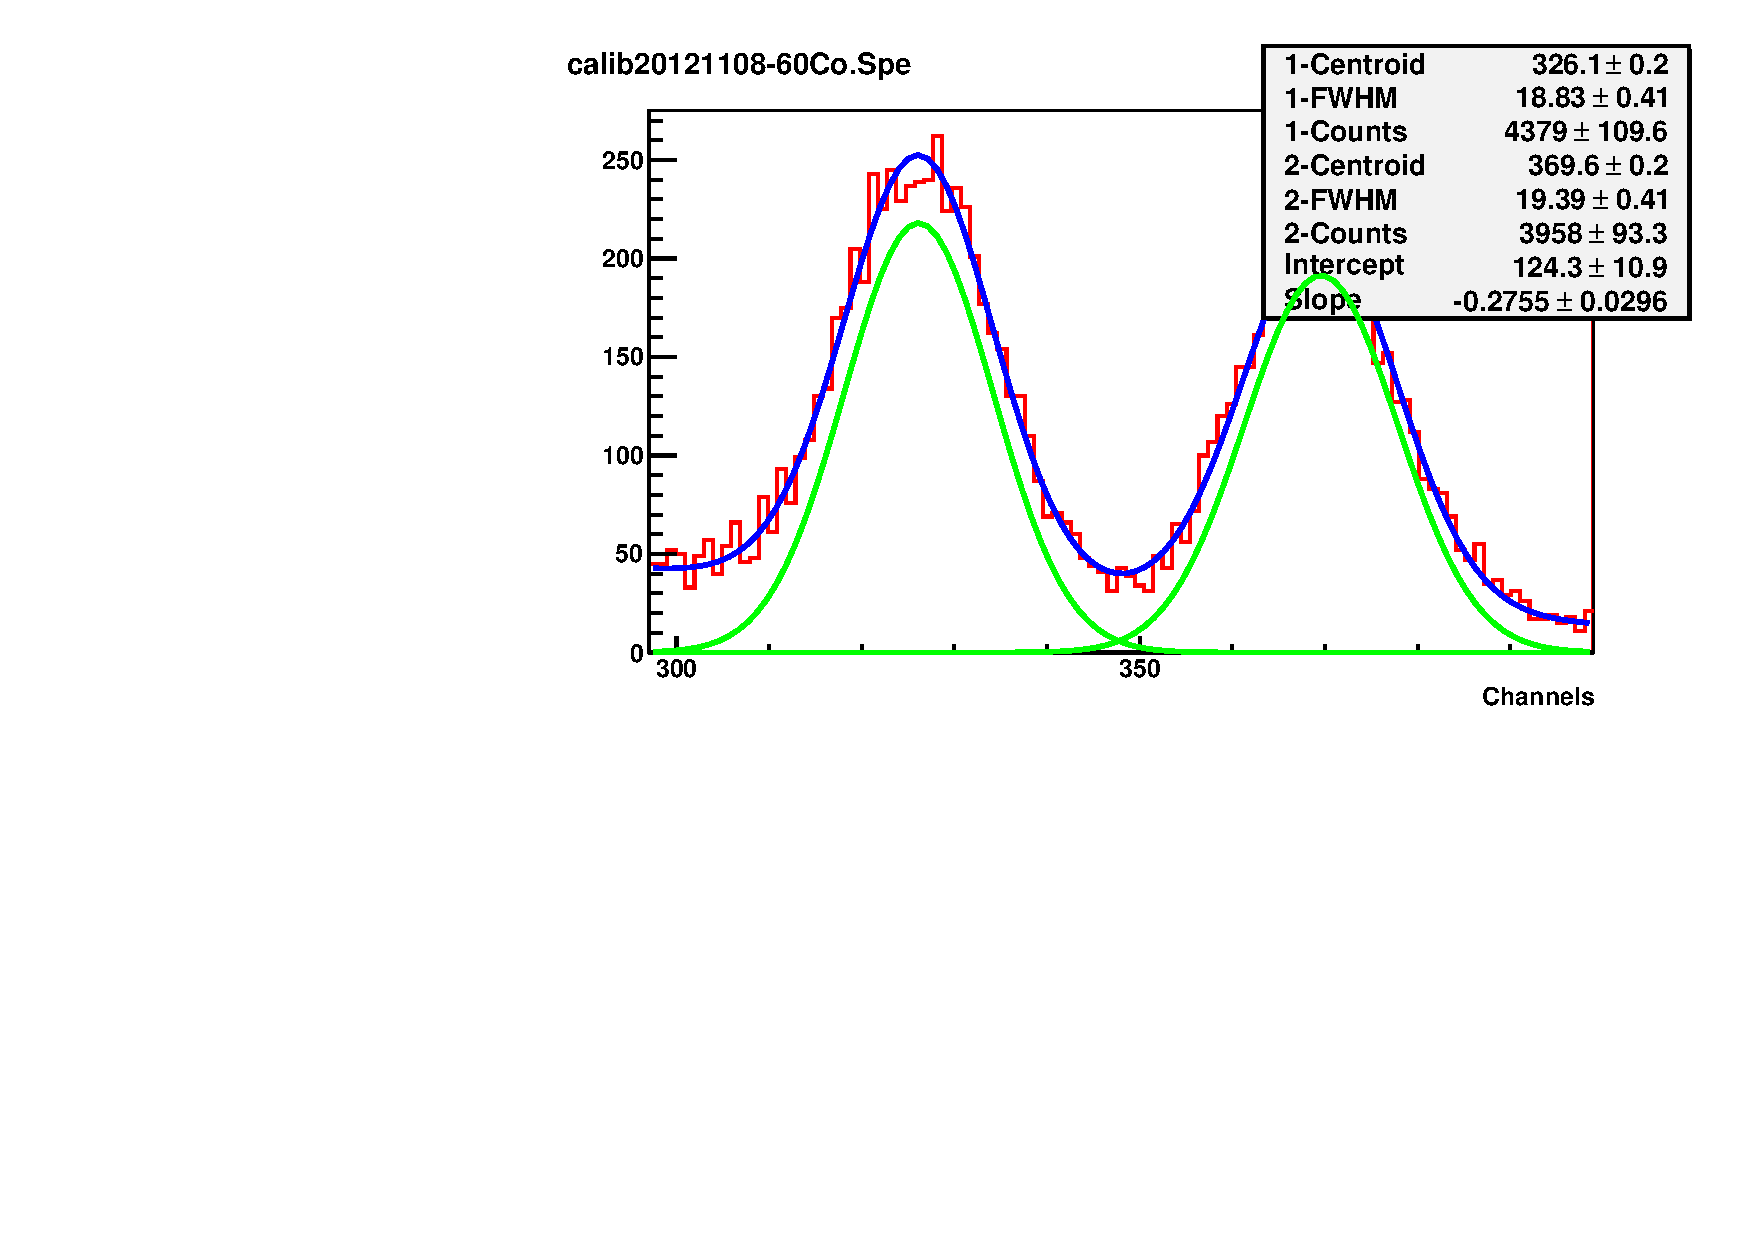
\includegraphics[width=0.7\textwidth]{calib20121113-60Co.pdf}
	\caption{An example of the peak for the radioactive element cobalt-60. These two peaks are well defined and have well known values. This means that they are good for using as calibration points for the detector.\label{fig:cobaltcalib}}
\end{figure}

This line has the equation,
\begin{align}
	E &= 3.63\times x - 18.31 \label{eq:calibNaI}
\end{align}
This equation, equation~\ref{eq:calibNaI}, shall be used as the calibration equation for the sodium iodide experiment. The calibration was re-taken at the start of each session using the NaI detector, so this value represents the session where the actual experimental results were taken for the main section of finding the deuteron binding energy.
% subsection calibration (end)

\subsection{Energy Resolution} % (fold)
\label{sub:energy_resolution}
Scintillation detectors, such as the NaI detector in use here, have a relatively poor energy resolution. Statistical broadening of the peaks is usually the dominant form of broadening. When a reaction takes place, and so energy is deposited, in the scintillator crystal, the efficiency can be as low as around 10\%. This means that a far smaller amount of energy is actually transferred to the crystal than the energy of the incoming particle.

When the reaction takes place in the crystal, a number of photons, proportional to the energy deposited, are produced. But some of them are lost before they can reach the photomultiplier tube further reducing the measured number of photons. This also means that there is a minimum in the number of photons just before the photomultiplier tube. Since the number of arriving photons will be subject to statistical fluctuations, the standard deviation in the photons reaching the PM tube is given by equation~\ref{eq:standarddevgamma}\cite{krane},
\begin{align}
	\text{Standard Deviation, }\sigma &= \sqrt{\text{Number of photons reaching the PM tube}}\label{eq:standarddevgamma}.
\end{align}
Since this is proportional to the energy of the original photon that caused the reaction, it can be shown that
\begin{align}
	R &= \frac{\text{FWHM}}{H_0} \\
	&= k\frac{\sqrt E}{E} = \frac{k}{\sqrt E}
\end{align}
Where FWHM is the full width at half maximum of any given peak, $H_0$ is the height of the peak and $k$ is a constant of proportionality. This means that the resolution can be easily observed by plotting a graph of $\log k$ against $\log E$, which should give a slope of $-\frac{1}{2}$ in an ideal case.

The resolution of the NaI detector was measured using the method described above.
% subsection energy_resolution (end)

\subsection{Neutron Binding Energy} % (fold)
\label{sub:neutron_binding_energy}
The first full experiment that was attempted was measuring the binding energy of neutrons by observing the $\gamma$-ray emitted when the neutrons are captured by protons in the water surrounding a neutron source via reaction~\ref{eq:neutronbinding},
\begin{align}
	\cf{^{1}_{1}p} + \cf{^{0}_{1}n} &\rightarrow \cf{^{1}_{2}d} + \gamma \label{eq:neutronbinding}
\end{align}

The exact energy would be found from the peak from this photon observed in the spectrum.

In order to observe the spectrum as clearly as possible, the experiment was run overnight collecting data for approximately 25 hours. This would give us a much clear spectrum and so lower errors on the final data. The spectrum that was recorded is shown in figure~\ref{fig:tank-full_spectrum}, along with a description of each of the major peaks that are visible. This plot is shown on a single $\log y$ axis so that the peaks are more easily discernible.
% \begin{figure}[ht]
% 	\centering
% 	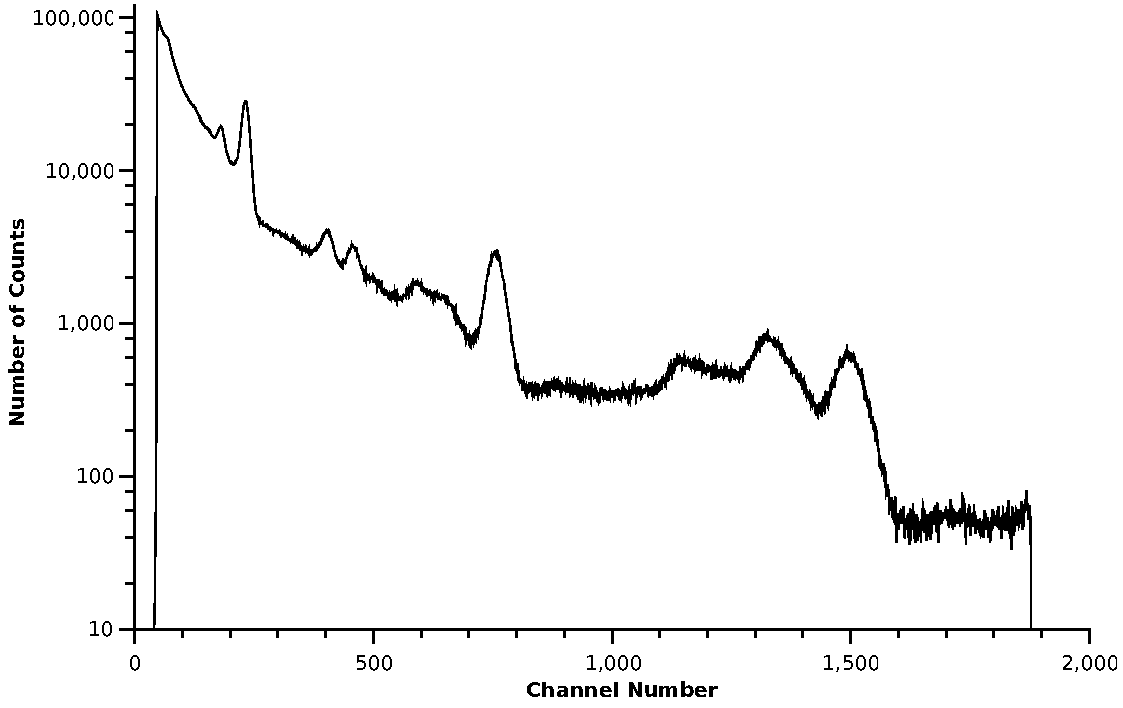
\includegraphics[width=0.9\textwidth]{tank-full_spectrum.pdf}
% 	\caption{The spectrum from the neutron tank observing a radioactive neutron emitter for a prolonged period.
% 	\label{fig:tank-full_spectrum}}
% \end{figure}
% \begin{figure}[ht]
%   \centering
%   \begin{overpic}[width=0.9\textwidth]{tank-full_spectrum.pdf}
%     \put(22,54){1}
%     \put(19,52.5){2}
%     \put(28,43){3}
%     \put(32,42){4}
%     \put(45,41){5}
%     \put(40,38){6}
%     \put(36,39){7}
%     \put(76,33){8}
%     \put(68,35){9}
%     \put(61,32){10}
%   \end{overpic}
%   \caption{The spectrum from the neutron tank observing a radioactive neutron emitter for a prolonged period of time.
%   \label{fig:tank-full_spectrum}}
% \end{figure}

\begin{figure}[ht]
  \centering
  \begin{overpic}[width=0.9\textwidth]{tank-full_spectrum_overnight.pdf}
    \put(20,57){1}
    % \put(19,52.5){2}
    \put(32,46){2}
    \put(36,44){3}
    \put(49,49){4}
    \put(44,43){5}
    \put(40,45){6}
    \put(85,36){7}
    \put(76,38){8}
    \put(66,36){9}
  \end{overpic}
  \caption{The spectrum from the neutron tank observing a radioactive neutron emitter for a prolonged period of time.
  \label{fig:tank-full_spectrum}}
\end{figure}

The major peaks, from figure~\ref{fig:tank-full_spectrum} are as follows:
	\begin{enumerate}\itemsep1pt \parskip0pt \parsep0pt
		\item 511\,keV peak from the electron rest mass.
		% \item Unknown.
		\item Unknown.
		\item Double escape peak?
		\item \textbf{Neutron binding energy}.
		\item Unknown
		\item Single escape peak from the neutron binding energy.\\
		Double escape peak from the neutron binding energy.
		\item Reaction peak from either oxygen ($\ce{^8O_2}$) or carbon ($\ce{^{12}C}$) from the water in the tank. Further investigation would be needed to determine the exact cause of this peak since it is so weak in comparison to the others.
		\item Escape peak from the carbon/oxygen peak
		\item Double escape peak from the carbon/oxygen peak
	\end{enumerate}

\subsubsection{Escape Peaks} % (fold)
\label{ssub:escape_peaks}
The peaks that are labelled as ``escape peaks'' from the previous graph, figure~\ref{fig:tank-full_spectrum}, are due to the phenomena called pair production. Pair production occurs if the incident energy is above 1022\,keV, i.e.\ twice the rest mass of the electron, and results in the production of two 511\,keV annihilation gamma rays. If one of these gamma rays escapes the detector while the other is completely absorbed, 511\,keV will be lost from the detector. This results in a separate peak in the spectrum representing the original energy minus 511\,keV. This is called a single escape peak. If both annihilation gamma-rays escape the detector a double escape peak is formed with an energy of the expected energy minus $2\times$ 511\,keV, or 1022\,keV\cite{baratta}.

Escape peaks can seen whenever there are events with energies greater than the 1022\,keV limit. They are generally slightly lower in height than the main peak and are always at the same distance from the main peak.
% subsubsection escape_peaks (end)

\subsubsection{Background Radiation} % (fold)
\label{ssub:background_radiation}
This experiment was carried out using a sample of americium-beryllium (AmBe) and as such, the peaks seen in the resulting spectrum should be well known and well defined. Instead, there are a number of peaks that cannot, at the present time, be accounted for. There are several explanations to explain these peaks. 
\begin{enumerate}
	\item The first is the method of creating the samples in use. The samples were made by bombarding the metals using a synchrotron particle accelerator. This has the effect of possibly creating an impure sample so that there are other elements that are decaying producing their own spectrum that is adding the the expected one.
	\item Another possibility is that the other radiation sources that are stored nearby introduced extra peaks from their own radioactive decays.
\end{enumerate}
% subsubsection background_radiation (end)

\subsection{Experimental Results} % (fold)
\label{sub:experimental_results}
The calibration data that was taken gave a channel number-energy relation of
\begin{align}
	E &= 3.63\times C - 18.31
\end{align}
where $E$ is the actual energy and $C$ is the observed channel number. Using this equation, peak number 5 from the above spectrum, figure~\ref{fig:tank-full_spectrum}, is found to lie at an energy of $2.244\pm0.048$\,MeV. The data taken from the spectrum is shown in table~\ref{tab:tankdata}. This table shows the channel number of each of the peaks labelled above, the error on this position, the energy and corresponding error for the peak and the differences between some of the adjacent peaks. This last column is used to verify escape peaks which are always at 511\,keV below the main peak.
\begin{table}[ht]
	\centering
	\begin{tabular}{c|c|c|c|c}
		Channel \textnumero & Error on Channel \textnumero & Energy & Error on Energy & Difference \\
		\hline\hline
		181.20 & 0.07 & 496 & 31 & \\
		232.45 & 0.02 & 651 & 32 &  \\
		403.33 & 0.15 & 1170 & 36 &  \\
		458.6 & 0.18 & 1338 & 38 &  \\
		617.3 & 0.56 & 1820 & 43 & 482 \\
		757.2 & 0.08 & 2244 & 48 & 425 \\
		1168.5 & 13.0 & 3492 & 66 & 1248 \\
		1335.4 & 0.50 & 3999 & 73 & 507 \\
		1496.6 & 0.28 & 4488 & 81 & 489
	\end{tabular}
	\caption{Values for the channel numbers and corresponding energies of the peaks from the spectrum of the BeAm sample in the water tank.\label{tab:tankdata}}
\end{table}

The values for the channel numbers, along with the corresponding errors, in table~\ref{tab:tankdata}, were taken from the results of the peak fitting algorithm, ``Buffit'', provided as an extension to be used with the ``root'' interpreter framework. An example of this peak fitting is shown below in figure~\ref{fig:tankspecbuffit}.

The value for the errors on the energies calculated here are given equation~\ref{eq:caliberrors}.
\begin{align}
	\left(\sigma E\right)^2 &= \left(\sigma Ch\times m\right)^2 + \left(\sigma m\times Ch\right)^2 + \left(\sigma c\right)^2 \label{eq:caliberrors}	
\end{align}
where
\begin{description}
	\item[$\sigma E$] is the error on the energy
	\item[$Ch$] is the channel number from the detector
	\item[$m$] is the gradient of the line fit of the data
	\item[$c$] is the intercept of the line fit.
\end{description}

\begin{figure}[ht]
	\centering
	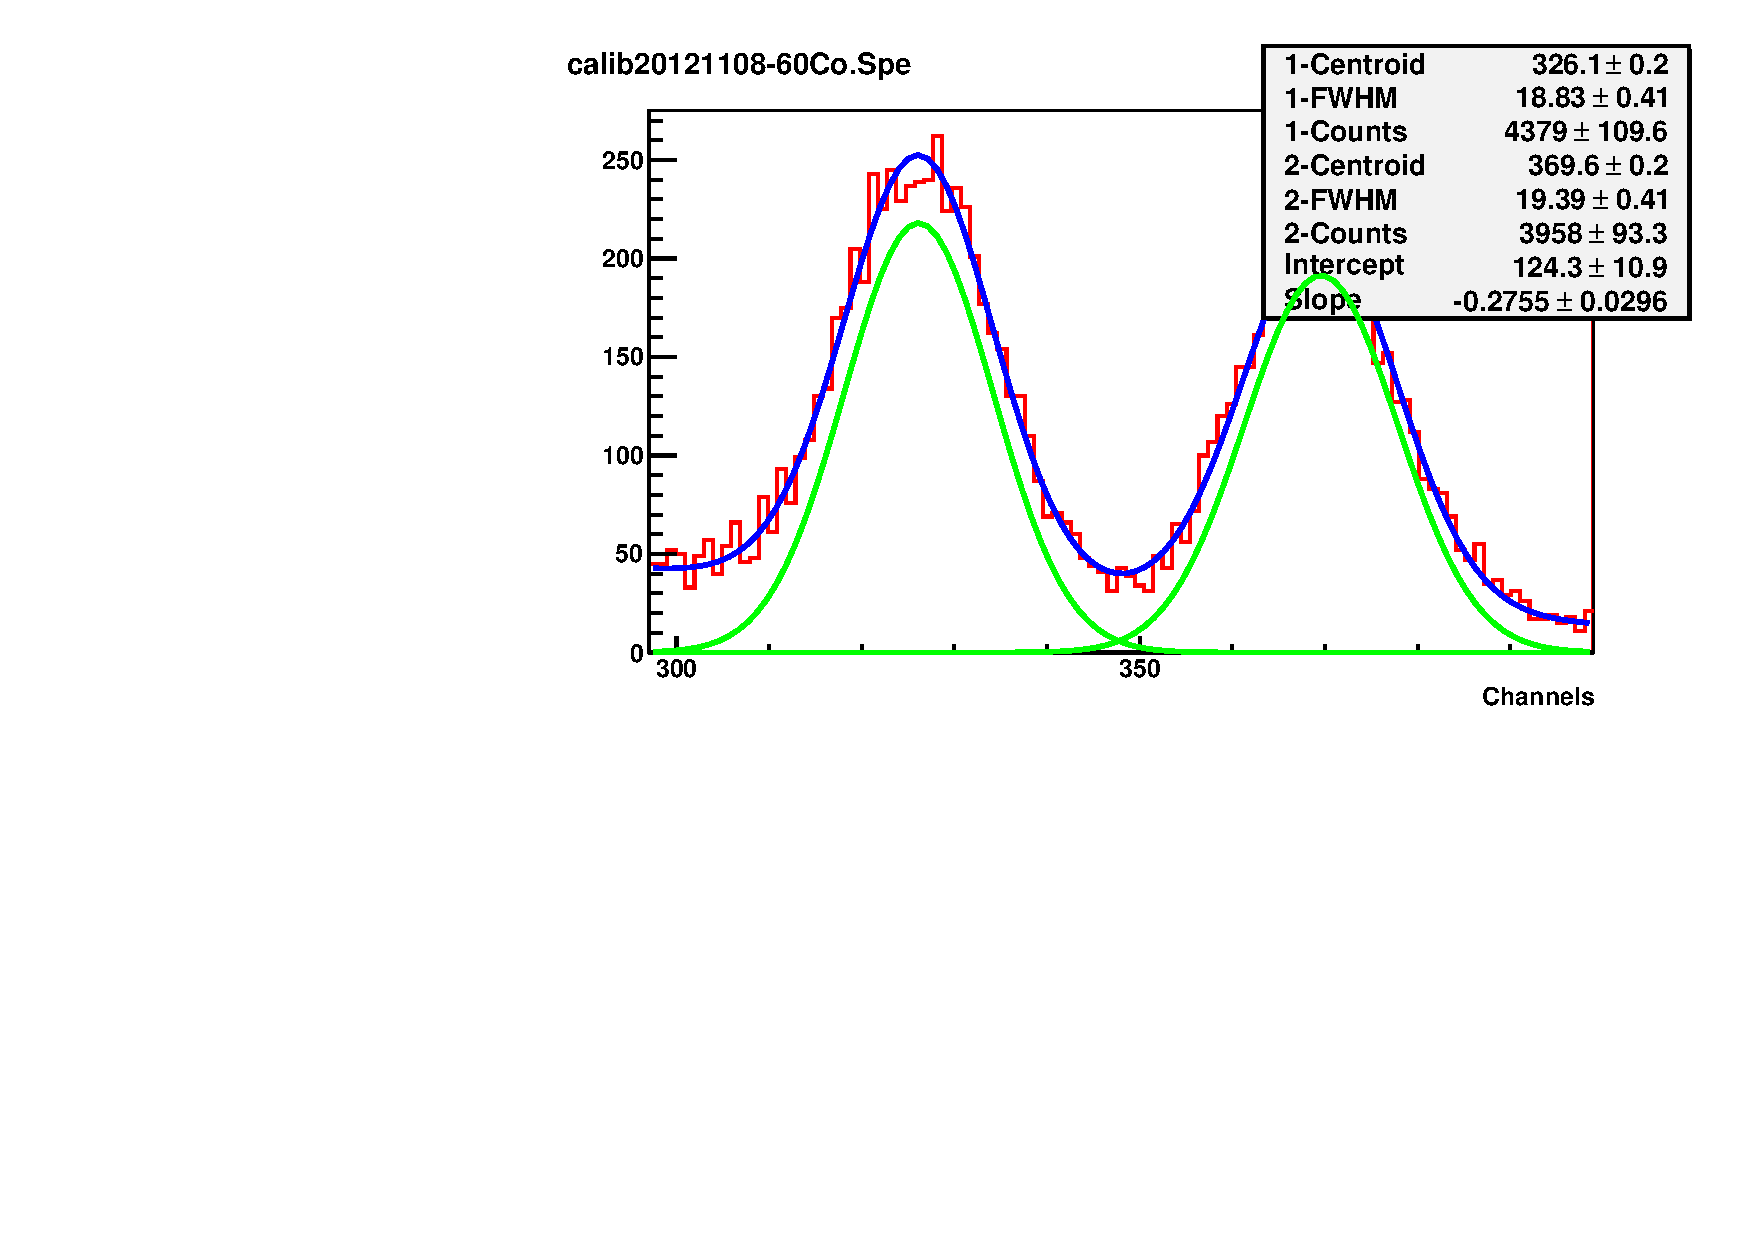
\includegraphics[width=0.7\textwidth]{calib20121113-60Co.pdf}
	\caption{An example of the peak for the radioactive element cobalt-60. These two peaks are well defined and have well known values. This means that they are good for using as calibration points for the detector.\label{fig:tankspecbuffit}}
\end{figure}

% subsection experimental_results (end)

\subsection{Analysis of Experimental Results} % (fold)
\label{sub:analysis_of_experimental_results}
The binding energy of the deuteron can be found theoretically from the mass difference between the deuteron and its individual components, as follows.
\begin{align}
	\ce{^1_0 n} + \ce{^1_1 p} &\rightarrow \ce{^2_1 d} + \gamma
\end{align}
The mass excess of each of these is as follows
\begin{align*}
	\Delta \ce{^1 p} &= 7.2889 \text{MeV} \\
	\Delta \ce{^1 n} &= 8.0713 \text{MeV} \\
	\Delta \ce{^2 d} &= 13.1357 \text{MeV}.
\end{align*}
The binding energy is thus
\begin{align}
	7.2889 + 8.0713 + 13.1357 &= 2.2245 \text{MeV}.
\end{align}
We can also find the difference between the binding energy of $\ce{^{16}O}$ and $\ce{^{17}O}$ from
\begin{align}
	\ce{^{16}_8 O} + \ce{^1_0 n} \rightarrow \ce{^{17}_8 O} + \gamma.
\end{align}
For this reaction, the mass excesses are
\begin{align*}
	\Delta \ce{^{16} O} &= -4.7370 \text{MeV} \\
	\Delta \ce{^{17} O} &= -0.8087 \text{MeV} \\
	\Delta \ce{^1 n} &= 8.0713 \text{MeV}.
\end{align*}
This confirms that the peak labelled number 4 is indeed in the correct energy location to be the binding energy of the neutron, and provides good evidence that the final unknown peak, peak number 7, could be from the oxygen in the water in the tank.
% subsection analysis_of_experimental_results (end)
% subsection neutron_binding_energy (end)

% section neutron_binding_energy (end)


%!TEX root = main.tex
\section{Neutron Attenuation In Water} % (fold)
\label{sec:neutron_attenuation_in_water}

\subsection{Boron Tri-Flouride Detector} % (fold)
\label{ssub:boron_tri_flouride_detector}
The BF$_3$ detector is a proportional counter. It contains boron trifluoride gas at 0.5 to 1 atmospheres which acts as both a target for slow neutron conversion into secondary particles, as well as a proportional gas. A large potential difference is applied across the gas. The cathode which is held at ground is the outer tube of the detector and is generally made from aluminium since this has a low neutron absorption cross section so should not influence any readings made by the detector. The anode, at high voltage, is a single wire that passes through the centre of the detector, see figure \ref{fig:bf3detector}. When a neutron is incident in the reactor, one of the reaction below takes place.
\begin{align}
	\cf{^{10}_{5}B} + \cf{^{1}_{0}n} &\rightarrow \cf{^{7}_{3}Li} + \cf{^{4}_{2}\alpha} \label{eq:bf31}\\
	\cf{^{10}_{5}B} + \cf{^{1}_{0}n} &\rightarrow \cf{^{7}_{3}Li^*} + \cf{^{4}_{2}\alpha} \label{eq:bf32}
\end{align} 

The products of these two equations differ only by the energy of the lithium which, in some cases, is left in an excited metastable state with a slightly different energy. The relative probabilities of each reaction is 96\% for equation \ref{eq:bf31} and 4\% for equation \ref{eq:bf32}. The resulting ions that are created are attracted to the poles of the detector and so provide a voltage through it. This provides a signal which is sent to the processing computer. It should be noted that this detector cannot give any information of the energy of the neutron since the formation of the ions is independent of energy over a certain level. Instead, this detector is used simply as a counter to obtain a value for the number of neutrons hitting it in a specified time period. 
\begin{figure}[ht]
	\centering
	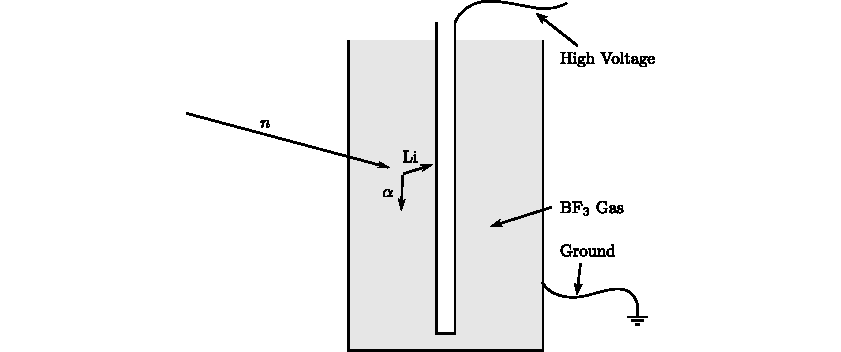
\includegraphics[width=0.9\textwidth]{BF3detector.pdf}
	\caption{The $\text{BF}_4$ detector uses a high charge to create a flow of ions to measure the incoming neutron. It cannot measure the energy, but simply gives a count for the number of neutrons incident in the detector. The anode and cathode create a large electric field inside the detector that creates the flow of charge used to count the incoming particles.\label{fig:bf3detector}}
\end{figure}

When the reaction happens, the products, $\cf{^7_3 Li}$ and $\cf{^4_2\alpha}$, are ejected through the BF$_3$ gas at a high velocity and can go on to cause further reactions in the gas as these ions deposit their kinetic energy. The electric field close to the wire increases quickly ($E\propto\frac{1}{r^2}$) and so a Townsend avalanche forms near to the wire when a reaction occurs. This involves the electrons being accelerated greatly by the electric field which causes the gas to conduct through the avalanche. The avalanche terminates when all of the free electrons reach the anode. These electrons produce the signal which is measured by the computer and used for analysis. Despite the several steps involved, if the detector is well designed, the number of electrons that is measured can be ensured to be proportional to the incident energy of the particles.

\subsubsection{Wall Effect} % (fold)
\label{ssub:wall_effect}
The BF$_3$ detector shall be used for several purposes later, so it is worth discussing some of the features of the data that is produced by this detector. Figure \ref{fig:walleffect2} shows a typical spectrum from the BF$_3$ detector. This shows a main peak, a smaller, higher energy secondary peak and an example of the wall effect.

When a neutron is incident with one of the atoms in the gas in the reactor, one of the reactions equation \ref{eq:bf31} or \ref{eq:bf32} takes place. If the reactor was extremely large compared to the travel distance of the Li and $\alpha$ products, then a single peak from each of the reactions would be observed, along with some amount of background noise, giving a spectrum similar to the top graph in figure \ref{fig:walleffect2}. The two peaks are from the reaction producing a ground state lithium atom or an excited lithium atom respectively. 
\begin{figure}[ht]
  \centering
  \begin{overpic}[width=0.8\columnwidth]{walleffect2.pdf}
    \put(57,48){2.31}
    \put(68,48){2.79}
    \put(25,25){Wall effect}
    \put(25,22){continuum}
    \put(30,20){\vector(0,-4){11}}
    \put(30,20){\vector(3,-2){12}}
    \put(65,40){$\text{Li}^* + \alpha$}
    \put(73,8){$\text{Li} + \alpha$}
    \put(46,12){$\alpha$}
    \put(32,9){Li}
  \end{overpic}
  \caption{An exemplar spectrum from the BF$_3$ detector showing the two peaks from each of the two reaction products, and the wall effect when one of the products from equation \ref{eq:bf31} escapes the detector.\label{fig:walleffect2}}
\end{figure}

The two steps in the count number at lower channel numbers is known as the wall effect. These are due to the detector being finite, or small compared to the travel distance of the reaction products, and so there is a chance that one of the products from the reaction escapes from the detector. Due to the relative masses of the particles created, $\alpha$ and Li, the $\alpha$ particle takes most of the energy from the original neutron and so when it is lost from the detector, the recoded energy is lower.

Other features of the spectrum are the abrupt cut-off at the low channel numbers. This is to reduce the background counts that are present in this region from obscuring the rest of the data. 
% subsubsection wall_effect (end)

\subsubsection{Boron Triflouride Detector Set-up} % (fold)
\label{ssub:boron_triflouride_detector_set_up}
Since it is only a proportional counter, and so gives no information for the energy of the observed particles, there is no calibration to be done with the BF$_3$ detector. However, there is a certain degree of adjustment that can, and should, be made to the settings of the detector before proceeding with the data acquisition. The detector requires a high voltage of between 1.4 to 2.6\,keV. This is the safe working range, but inside these limits, the voltage that gives the clearest results can be chosen. Figure \ref{fig:bf3voltages} shows several graphs from the BF$_3$ detector using different voltages to ascertain which would be the most appropriate voltage to use.
\begin{figure}[ht]
  \centering
  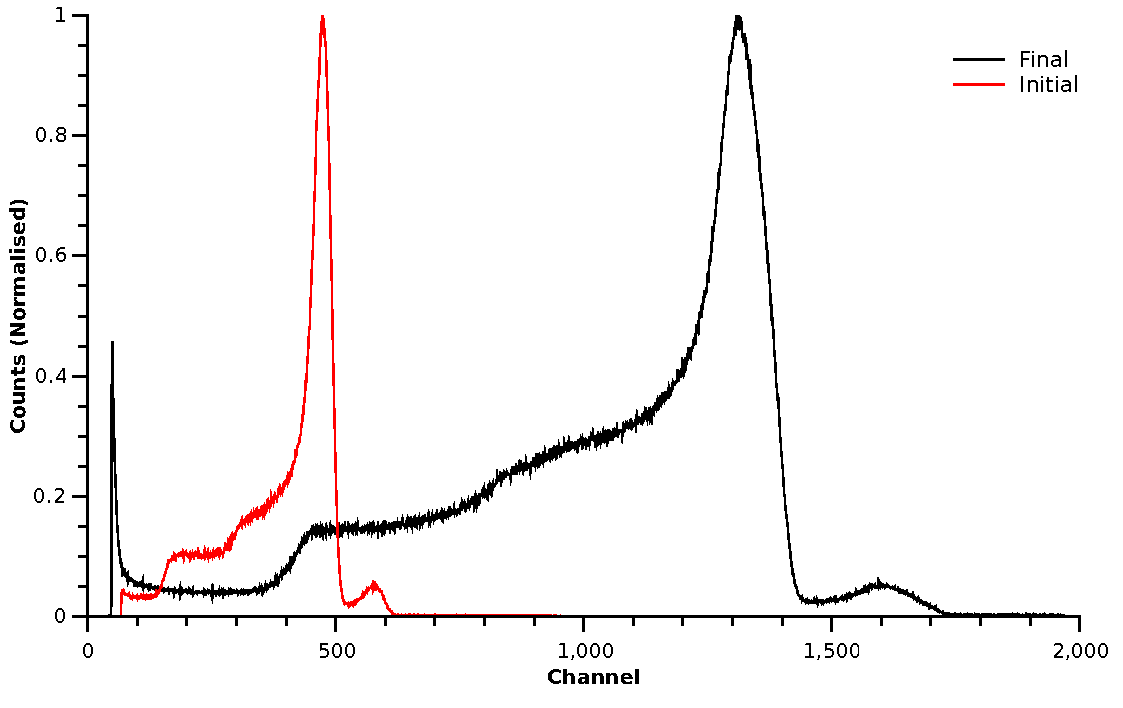
\includegraphics[width=0.6\textwidth]{BF3_calib_voltage.pdf}
  \caption{The effect of adjusting the supplied voltage correctly. The initial readings, using the lower bound of the allowed voltage range does not make full use of the channel range and so any readings will be subject to higher errors. The final voltage level that was used takes full advantage of the channel width of the detector. \label{fig:bf3voltages}}
\end{figure}
% subsubsection boron_triflouride_detector_set_up (end)

% subsubsection boron_tri_flouride_detector (end)
\subsection{Neutron Attenuation} % (fold)
\label{sub:neutron_attenuation}In order to examine the attenuation effects of water to neutrons from the beryllium-americium source, the spectrum of neutrons will be measured with the BF$_3$ detector at a range of distances from the source, moving radially outward through the water. The readings shall be taken for precisely the same length of time using the built in timing function of the software used to record the readings. The count value from the data will be taken from the centre of the lower wall upwards, since everything below this point must be background radiation.

An estimate for the background radiation involved in the main section of the readings can also be made. By looking at the spectrum recorded from the detector, it can be seen that the background level just prior to the first wall, and so before any useful information from either reaction, and just after the second peak, can be joined by a straight line, representing a linear falloff of background across the channels. This is shown in figure \ref{fig:bf3errorest}. The count number represented by this triangle can be measured, and subtracted from the total count, which shall also be taken inside these limits. This should provide a reduced count number that has removed a significant proportion of the background that would have affected the result.
\begin{figure}[ht]
  \centering
  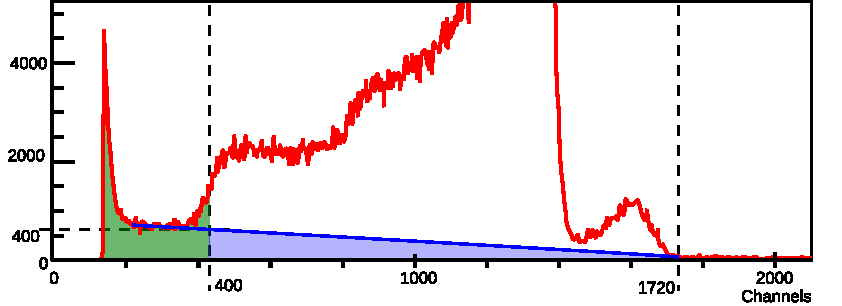
\includegraphics[width=0.8\textwidth]{BF3background.pdf}
  \caption{An estimate of the background is made by assuming it falls linearly from the beggining of the channel numbers, which has to be error, to a point where it is known to be zero, after the second peak. The green shaded region is known to background since the second step represents the loss of both the lithium and the $\alpha$ particles. \label{fig:bf3errorest}}
\end{figure}

The total number of counts is a function provided by the software that is used, called Maestro. This allows us to easily record the number of counts for specific regions of the graph. Using this method, and initial trial recording was taken to work out an estimate for the percentage of the total counts were contributed by this background radiation. Equation \ref{eq:backgroundcalc} shows the calculation used to calculate the background,
\begin{align}
  (1729-400)\times 400 \times 0.5 &= 264,000\,\text{counts} \label{eq:backgroundcalc}
\end{align}
The total counts, including this noise, was $3.82\times10^6$, hence, the background represents roughly 6.9\% of the total counts.
% subsection neutron_attenuation (end)
\subsection{Experimental Results} % (fold)
\label{sub:bf3experimental_results}

% subsection experimental_results (end)
\subsection{Neutron Attenuation Theory} % (fold)
\label{sub:neutron_attenuation_theory}
In order to model the situation, in a simplified way, the statistical one-group approach is used. It shall be assumed that all of the neutrons are thermalised, reduced in speed to similar to the surrounding particles, and an estimate for the diffusion length can be found. The diffusion length is the distance a thermal, or fast travelling neutron, takes to slow down. Once it has been thermalised, the neutron can be absorbed by matter, for example, an oxygen atom in the water surrounding the source. Thermalisation is the best method for reducing the speed of neutrons for many applications, since neutrons are not charged particles and so do not interact with electric or magnetic fields.

The Americium-Beryllium source that was used was assumed to be a point source, which is a good approximation compared with the distances that we are measuring, and so the emitting of neutrons from such a source is given by
\begin{align}
  \dx{n}{t} &= -\Sigma_a \phi - \div{J} \label{eq:neutronflux}
\end{align}
where $n$ is the number of neutrons at time $t$, $\Sigma_a$ is the absorption cross section of the water in the tank, $\phi$ is the neutron flux (number of neutrons travelling through a unit are in unit time) and the vector $\textbf{J}$ is the diffusion flux from Fick's law shown in equation \ref{eq:fick},
\begin{align}
  \textbf{J} = - \textbf{D}\grad\phi \label{eq:fick}
\end{align}
This means that the term from equation \ref{eq:neutronflux}, $-\Sigma_a\phi$ is the loss of neutrons due to absorption, and the term $-\div{\textbf{J}}$ is the divergence. Since the flux is simply the number passing a static point multiplied by their velocity, $\phi = nv$, equation \ref{eq:neutronflux} can be written as
\begin{align}
  \frac{1}{v}\dx{\phi}{t} &= -\Sigma_a\phi + D\laplacian\phi^2
  \intertext{But in the steady state, $\dx{\phi}{t} = 0$, so}
  \Sigma_a\phi &= D\laplacian\phi
\end{align}
The region of interest around the source, the water tank filled with water, has cylindrical symmetry but also, up to a radius of roughly 0.5\,m has spherical symmetry. In this case, the neutron flux is independent of the angle measured at and so this equation can be simplified to to a single dimension.
\begin{align}
  \frac{1}{r^2}\frac{\text{d}}{\text{d}r^2}\left( r^2\dx{\phi_r}{r} - \frac{1}{L^2}\phi_r \right) &= 0 \label{eq:diffusion}
\end{align}
  where the diffusion length, L, which is the distance travelled by an average neutron through the water, is given by
\begin{align}
  L &= \sqrt{\frac{D}{\Sigma_a}}.
\end{align}
The solutions of the equation \ref{eq:diffusion} have the form
\begin{align}
  \phi &= A\frac{e^{-\frac{r}{L}}}{r} + B\frac{e^{\frac{r}{L}}}{r}
\end{align}
To simplify this equation, it is assumed that the coefficient, $B$, is zero, since otherwise the second term would tend to infinity as the radius increases, which is clearly un-physical. This leaves the following equation
\begin{align}
  \phi &= A\frac{e^{-\frac{r}{L}}}{r} \\
  r\phi &\propto e^{-\frac{r}{L}}
\end{align}
Thus, when $\ln(r\phi)$ is plotted against $r$, the graph should have a gradient of $-\frac{1}{L}$
% subsection neutron_attenuation_theory (end)
% section neutron_attenuation_in_water (end)


%!TEX root = main.tex
\section{Conclusion} % (fold)
\label{sec:conclusion}
This experiment was designed to investigate two phenomena using a Beryllium-Americium source and a pair of nuclear detectors. The first was to make a measurement of the binding energy of the deuteron by observing the $\gamma$-ray emitted when neutrons are captured by protons in the water surrounding a neutron source via the reaction 
\begin{align}
	p + n \rightarrow d + \gamma.
\end{align}
This was found to have a value of 2.2245\,MeV which is very close to the accepted value of $2224.52\pm 0.20$\,keV. The measurement of the deuteron binding energy was very successful, however, the preliminary experiments to investigate the detector itself, to determine its energy resolution and efficiency by looking at samples with known well defined peaks was less successful. 

Problems were encountered when plotting the data that had been acquired suggesting that it was not accurate enough to draw any firm conclusions possibly because of the errors that had been introduced during measurement. There was often a general trend in the data as would be expected, but the points were too scattered to be able to fit the data to the mathematical model. For example, when looking at the efficiency of the sodium iodide detector, the plot in figure~\ref{fig:NaIefficiancy} was measured.
\begin{figure}[ht]
	\centering
	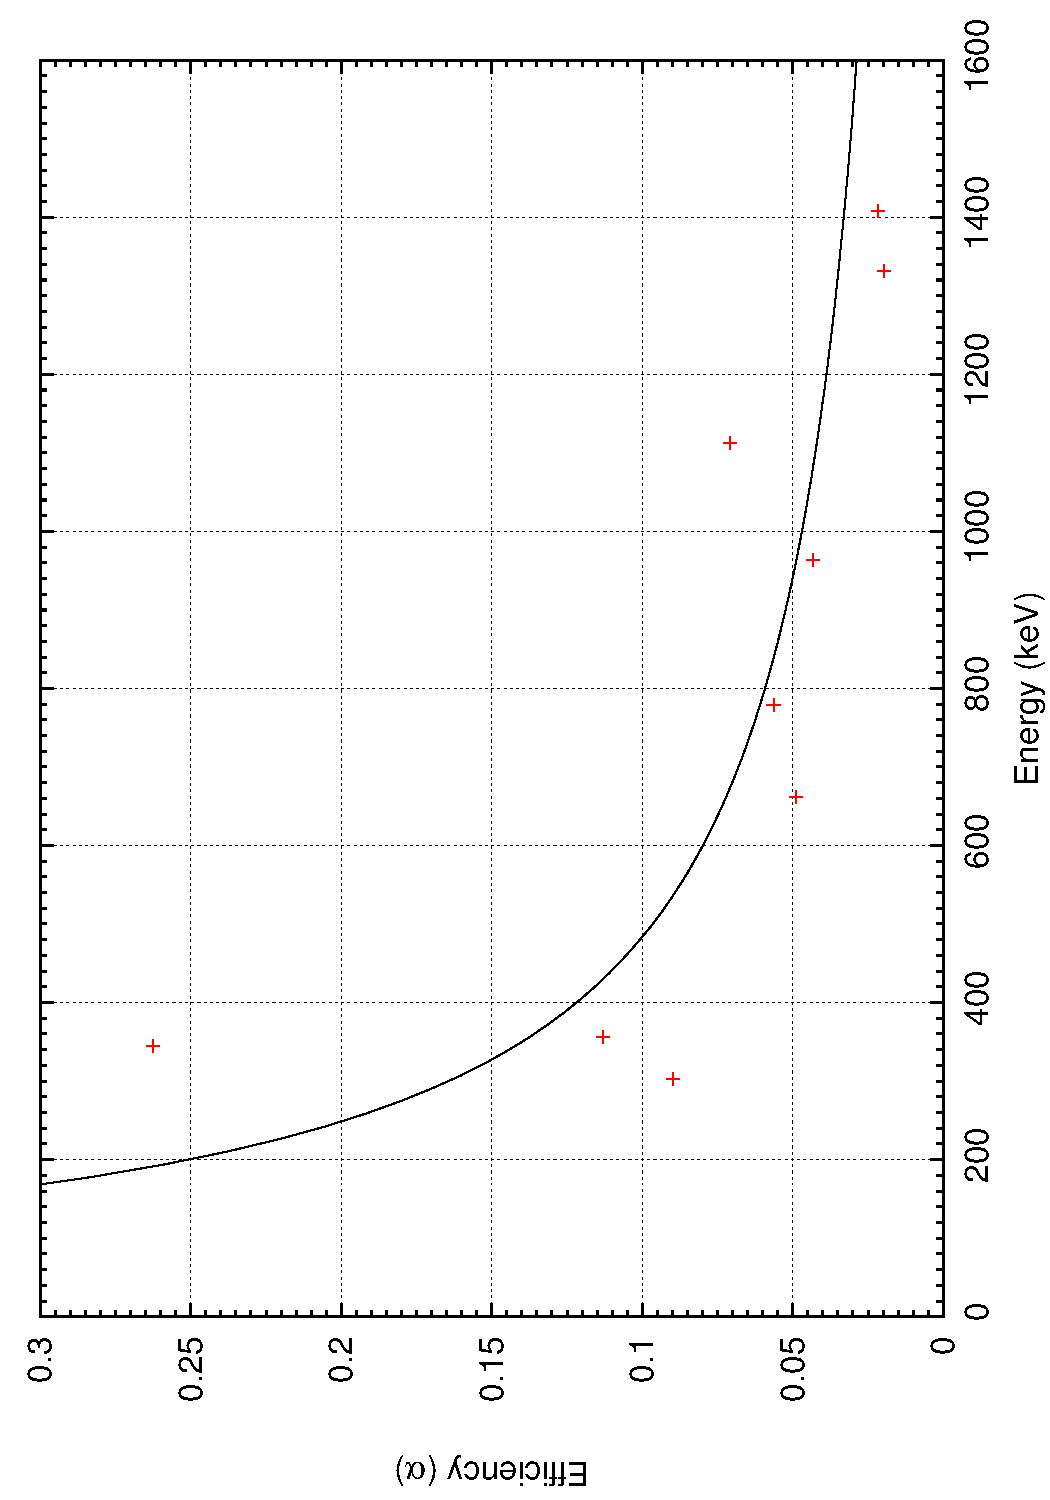
\includegraphics[angle=270,width=0.6\textwidth]{NaIEfficiency.pdf}
	\caption{The sodium iodide detector provides a channel number readout that is directly proportional to the energy of the corresponding reaction event. Thus, using known data points, a relation between channel number and energy can be found.\label{fig:NaIefficiancy}}
\end{figure}
Though this is a poor fit, as the data points are not closely matched to the line, we can confirm that the general trend in the efficiency as the energy increases is correct, as can be seen in the diagram in figure~\ref{fig:efficiencyKrane}\cite{krane}.
\begin{figure}[ht]
	\centering
	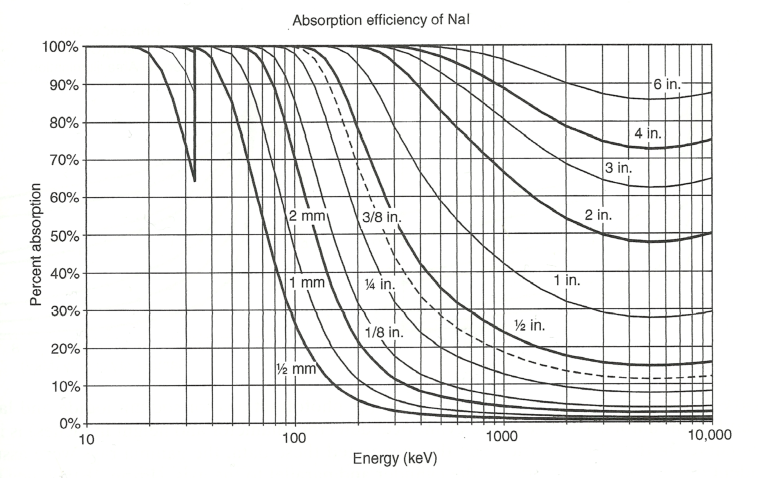
\includegraphics[width=0.7\textwidth]{EfficiencyKrane.pdf}
	\caption{The sodium iodide detector provides a channel number readout that is directly proportional to the energy of the corresponding reaction event. Thus, using known data points, a relation between channel number and energy can be found.\label{fig:efficiencyKrane}}
\end{figure}

The second experiment involved using a boron triflouride detector to measure the moderating effect of water on the neutrons observed from a BeAm source. For this we found that there were several elements of the spectra that were observed that had to be understood in order to measure the moderating effects fully. These included the wall effect and the contribution of the background radiation to the readings made by the proportional counter. 

Once these elements were understood, we were able to take measurements of the neutron flux at increasing radii from the source, moving out through the tank filled with water. We found that the majority of the data followed the expected trend provided by the one-group equation describing the thermalization of neutrons in the water tank.
% section conclusion (end)


%!TEX root = mainfile.tex

%\bibliographystyle{plain}
\bibliography{yourbib.bib}{}
\cleardoublepage


\end{document}
    
 
%   \caption{\label{fig:quantumerror}Even with just three qubits, the encoding power is much higher. The cumulative effect of increasing the number of qubits is huge.}
% \end{figure}

Also, from here, the html files can be chosen, as can the images used in the book. Tabs are used to keep the interface clean and less cluttered. The file chooser that is opened when the button to select the files is clicked is an FLTK built in file chooser.

Below these entry boxes are the main controls for the program. ``Exit'' closes the window and ends the application, ``Refresh'' updates the in application information about the book to reflect and changes made by the user, and ``Create!'' takes the entered information and writes it to the relevant files. It also copies the selected files from the location chosen to the temporary folder used by the application. Once this has finished, it ZIPs the resulting folder as specified in the document specification and names it according the user's choice of name for the book.

Next to the input boxes, on the right side of the window, are a number of tabs that inform the user what will be written when they click the create button to make their book. These tabs provide information for those interested in the structure of epub ebooks and provide a means of checking that the book will be created as expected. Each separate tab contains what will be included in each of several separate files (see figure \ref{fig:structure}).

At the top of the window, there is a menu bar with a few options and operations. These include buttons that perform the same functions as the buttons previously mentioned, exit, update and create as well as the ``About'' dialogue, shown in figure \ref{fig:about}, and an option to set the current operating system (see below for details).
\begin{figure}[ht]
  \centering
  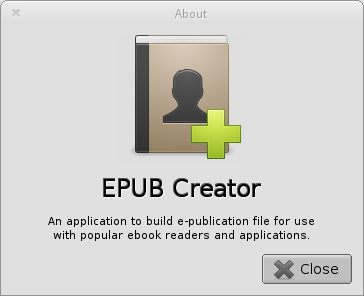
\includegraphics[width=0.35\columnwidth]{about.png}
  \caption{\label{fig:about}The ``About'' window provides information about the application and could be extended to include licensing information, bug reporting information and developer details etc.}
\end{figure}

\subsection{Internal Structure}
The code for this project is shown at the end of this document in appendices \ref{app:code1} through \ref{app:code9}. The project started as a single long file with all of the various functions distributed throughout. I took the decision to split the code through several files that are interdependent, but which contain a smaller subset of the code, grouped according to the function that it achieves. Each of the files is used by one or more other files, the include tree is shown in figure \ref{fig:files}.
\begin{figure}[ht]
  \centering
    \inputTikZ{files}
  \caption{\label{fig:files}A diagram showing the structure of the epub project files and their interdependencies.}
\end{figure}

The most important aspect of the code is the class called ``Meta''. This contains all of the variables and the associated functions that make up and allow interaction with a book. Meta stands for meta-data which includes information like the title, author and language as well as more extensive information, like the contents of the static files for inclusion in the final book. The class contains these data, as well as the means to access and modify them.

\section{Critique}
The aim of this project was to build an application to aid in the building of ebook according to the specification written by the IDPF. This, the application achieves. You are able to select the pre-written files, include them in the document and specify the details about the document that you wish, or are required, to be specified. It also has some flexibility so that the number and type of included text files does not matter, and man or no images can be selected.

However, there are several areas where this application would require more work and possibly redesign were it to be used on a larger scale. Some of these that I have identified are listed below.
\begin{itemize}
  \item There is no way to rearrange the files that are included so that they are added to the book in the right order (the only way currently is to name the files sequentially as the file chooser adds the files to the array in alphanumerical order).
  \item Some of the elements of the GUI do not behave as expected, for example on resize some of the buttons change location and/or size instead of remaining static and the space around them changing.
  \item To extend the functionality of the application, there are several features that could be added, such as:
    \begin{itemize}
      \item Front cover chooser,
      \item Text editor for main text files.
    \end{itemize}
  \item The code could be further compartmentalised into functions to simplify and reduce the repetition of elements.
\end{itemize}

\section{Notes} % (fold)
\label{sec:notes}
\begin{itemize}
  \item This application is written for the Linux operating system. Though it shall run under other operating systems, like Windows, the core functionality of the program require Linux. The program ``zip'', which is by default installed on almost all systems, is a requirement for this program to function properly. 
  \item Included in the files for the program is a makefile that can be used to build the program under the same Linux environment. This requires all of the files for the program to be in the same directory along with the makefile. The program can then be built using the command \code{make} from the terminal (alternatively use \code{make \&\& ./epub} to build and then run the program). This will create several directories as well as the program executable, ``epub''. Running \code{make clean} will remove the auxillary files that are created during the build process.
  \item Also included in the program files is a folder called ``Example'' which includes a set of html and image files that can be used to test the program. These are merely a web page that has been saved locally and been stripped of the JavaScript, CSS elements and some header information. To use this example, simply run the program  as usual and choose the relevant files from the 
\end{itemize}

% section notes (end)

\newpage
\appendix
\addcontentsline{toc}{section}{Appendix}

\definecolor{dkgreen}{rgb}{0,0.6,0}
\definecolor{gray}{rgb}{0.5,0.5,0.5}
\definecolor{mauve}{rgb}{0.58,0,0.82}
\lstset{ %
%  basicstyle=\scriptsize,         % the size of the fonts that are used for the code
  numbers=left,                   % where to put the line-numbers
  numberstyle=\tiny\color{gray},  % the style that is used for the line-numbers
  stepnumber=5,                   % the step between two line-numbers. If it's 1, each line will be numbered
  numbersep=5pt,                  % how far the line-numbers are from the code
  showspaces=false,               % show spaces adding particular underscores
  showstringspaces=false,         % underline spaces within strings
  showtabs=false,                 % show tabs within strings adding particular underscores
  frame=single,                   % adds a frame around the code
  rulecolor=\color{black},        % if not set, the frame-color may be changed on line-breaks within not-black text (e.g. comments (green here))
  breaklines=true,                % sets automatic line breaking
  breakatwhitespace=false,        % sets if automatic breaks should only happen at whitespace
  keywordstyle=\color{blue},      % keyword style
  commentstyle=\color{dkgreen},   % comment style
  stringstyle=\color{mauve},      % string literal style
}

\section*{Meta.h}
\label{app:code1}
\scriptsize\lstinputlisting[language=C++]{Meta.h}

\section*{Meta.cxx}
\label{app:code2}
\scriptsize\lstinputlisting[language=C++]{Meta.cxx}

\section*{about.h}
\label{app:code3}
\scriptsize\lstinputlisting[language=C++]{about.h}

\section*{about.cxx}
\label{app:code4}
\scriptsize\lstinputlisting[language=C++]{about.cxx}

\section*{epubfunctions.h}
\label{app:code5}
\scriptsize\lstinputlisting[language=C++]{epubfunctions.h}

\section*{epubfunctions.cxx}
\label{app:code6}
\scriptsize\lstinputlisting[language=C++]{epubfunctions.cxx}

\section*{epubmk.h}
\label{app:code7}
\scriptsize\lstinputlisting[language=C++]{epubmk.h}

\section*{epubmk.cxx}
\label{app:code8}
\scriptsize\lstinputlisting[language=C++]{epubmk.cxx}

\section*{epub2.cpp}
\label{app:code9}
\scriptsize\lstinputlisting[language=C++]{epub2.cpp}

\end{document}





